\begin{name}
	{\tenchude}{ĐỀ ÔN TẬP SỐ 7}{LỚP TOÁN THẦY PHÁT}{\thoigian}
\end{name}
\setcounter{ex}{0}
\setcounter{bt}{0}
\Opensolutionfile{ans}[ans/ans-Vted-17-2023]
%Lê Hồng Phi
%%==========Câu 1
\begin{ex}%[Lê Hồng Phi]%[Tex hóa Đề Vted 2023]%[2D4Y1-2]
	\immini{Trong hình vẽ bên, điểm $M$ biểu diễn số phức $z$. Số phức $\overline{z}$ là 
		\choice
		{$1-2i$}
		{\True $2-i$}
		{$2+i$}
		{$1+2i$} }{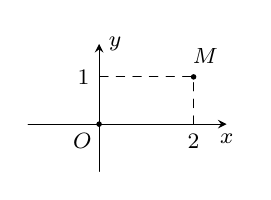
\begin{tikzpicture}[scale=1, font=\footnotesize, line join=round, line cap=round,>=stealth,x=0.6cm,y=0.6cm]
			\def \xmin{-1.5};
			\def \xmax{2.7};
			\def \ymin{-1.};
			\def \ymax{1.7};
			\draw[->] (\xmin, 0.) -- (\xmax,0.) node[anchor=north] {$x$};
			\draw[->] (0.,\ymin) -- (0.,\ymax) node[anchor=west] {$y$};
			\clip (\xmin+0.1,\ymin+0.1) rectangle (\xmax-0.1,\ymax-0.1); 
			\draw[dashed] (2,0) node[below]{$2$} |- (0,1)node[left]{$1$};
			\foreach \x/\y/\l/\g  in {0/0/O/225,2/1/M/60}{\fill[black] (\x,\y) circle(1pt)+(\g:0.5) node{$\l$};}
	\end{tikzpicture}}
	
	\loigiai{
		Theo hình vẽ, điểm $M$ biểu diễn số phức $z=2+i$.\\
		Vậy $\overline{z}=2-i$.
	}
\end{ex}

%%==========Câu 2
\begin{ex}%[Lê Hồng Phi]%[Tex hóa Đề Vted 2023]%[2H1Y3-2]
	Thể tích của khối chóp đều $S.ABCD$ có độ dài cạnh đáy bằng $2a$, chiều cao bằng $3a$ là
	\choice
	{$18a^3$}
	{$12a^3$}
	{\True $4a^3$}
	{$6a^3$}
	\loigiai{
		\immini{Diện tích hình vuông $ABCD$ là $S_{ABCD}=(2a)^2=4a^2$.\\
			Vậy thể tích của khối chóp đều $S.ABCD$ là $$V=\dfrac{1}{3}\cdot S_{ABCD}\cdot h=\dfrac{1}{3}\cdot4a^2\cdot 3a=4a^3.$$}{\begin{tikzpicture}[scale=1, font=\footnotesize, line join=round, line cap=round,>=stealth]
				\path (0,0)coordinate (B) (3,0) coordinate (C) (4.5,1) coordinate (D) ($(B)+(D)-(C)$) coordinate (A) ($(A)!0.5!(C)$) coordinate (O) (0,2.5) coordinate (h) ($(O)+(h)$) coordinate (S);
				\draw (S)--(B)--(C)--(D)--cycle (S)--(C);
				\draw[dashed] (O)--(S)--(A)--(B) (C)--(A)--(D)--(B);
				\foreach \p/\g in {A/150,B/240,C/-60, D/0, S/90,O/-90} \fill[black] (\p) circle(1pt)+(\g:0.3) node{$\p$};
		\end{tikzpicture}}
	}
\end{ex}

%%==========Câu 3
\begin{ex}%[Lê Hồng Phi]%[Tex hóa Đề Vted 2023]%[2D1B5-5]
	\immini{Cho hàm số $f(x)$ có đồ thị của đạo hàm như hình vẽ bên. Hàm số $f(x)$ đồng biến trên khoảng nào dưới đây?
		\choice
		{$(1;3)$}
		{\True $(-\infty;0)$}
		{$(0;1)$}
		{$(3:+\infty)$}
	}{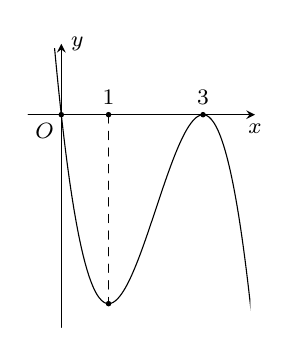
\begin{tikzpicture}[scale=1, font=\footnotesize, line join=round, line cap=round,>=stealth,x=0.6cm,y=0.6cm]
			\def \xmin{-0.7};
			\def \xmax{4.1};
			\def \ymin{-4.5};
			\def \ymax{1.5};
			\draw[->] (\xmin, 0.) -- (\xmax,0.) node[anchor=north] {$x$};
			\draw[->] (0.,\ymin) -- (0.,\ymax) node[anchor=west] {$y$};
			\clip(\xmin+0.1,\ymin+0.1) rectangle (\xmax-0.1,\ymax-0.1);
			\draw[smooth,samples=100,domain=\xmin:\xmax] plot(\x,{-(\x-2)^3+3*(\x-2)-2});
			\draw[dashed] (1,0) node[above]{$1$} -- (1,-4) (3,0) node[above]{$3$};
			\foreach \x/\y  in {1/0,3/0,1/-4}{\fill[black] (\x,\y) circle(1pt);}
			\foreach \x/\y/\l/\g  in {0/0/O/225}{\fill[black] (\x,\y) circle(1pt)+(\g:0.5) node{$\l$};}
	\end{tikzpicture}}
	\loigiai{
		Từ hình vẽ ta có $f'(x)>0$ khi $x<0$.\\
		Vậy hàm số $f(x)$ đồng biến trên  khoảng $(-\infty;0)$.
	}
\end{ex}

%%==========Câu 4
\begin{ex}%[Lê Hồng Phi]%[Tex hóa Đề Vted 2023]%[2H3Y3-1]
	Trong không gian  $Oxyz$, cho đường thẳng $d\colon \dfrac{x-1}{2}=\dfrac{z+1}{-1}=\dfrac{y-2}{3}$. Một véc-tơ chỉ phương của $d$ là
	\choice
	{\True $\overrightarrow{u}_1=(2;-1;3)$}
	{$\overrightarrow{u}_2=(-1;1;-2)$}
	{$\overrightarrow{u}_3=(-1;2;-1)$}
	{$\overrightarrow{u}_4=(2;3;-1)$}
	\loigiai{
		Một véc-tơ chỉ phương của $d$ là $\overrightarrow{u}_1=(2;-1;3)$.
	}
\end{ex}

%%==========Câu 5
\begin{ex}%[Lê Hồng Phi]%[Tex hóa Đề Vted 2023]%[2H3Y2-3]
	Trong không gian
	$Oxyz$, mặt phẳng toạ độ $(Oxy)$ có phương trình là
	\choice
	{\True $z=0$}
	{$x+y=0$}
	{$x=0$}
	{$y=0$}
	\loigiai{
		Mặt phẳng toạ độ $(Oxy)$ có phương trình là $z=0$.
	}
\end{ex}

%%==========Câu 6
\begin{ex}%[Lê Hồng Phi]%[Tex hóa Đề Vted 2023]%[2D1Y4-1]
	Tiệm cận ngang của đồ thị hàm số $y=\dfrac{1-2x}{x-1}$ là đường thẳng có phương trình
	\choice
	{$y=1$}
	{$y=2$}
	{\True $y=-2$}
	{$y=-1$}
	\loigiai{
		Tập xác định $\mathscr{D}=\mathbb{R}\setminus\{1\}$.\\
		Ta có $\lim\limits_{x\to +\infty}y=-2$, $\lim\limits_{x\to -\infty}y=-2$ nên đường thẳng $y=-2$ là tiệm cận ngang của đồ thị hàm số.
	}
\end{ex}

%%==========Câu 7
\begin{ex}%[Lê Hồng Phi]%[Tex hóa Đề Vted 2023]%[2H3Y1-2]
	Trong không gian  $Oxyz$, cho hai véc-tơ $\overrightarrow{u}=(1;-2;3)$ và $\overrightarrow{v}=(2;-2;1)$. Khi đó $\overrightarrow{u}\cdot\overrightarrow{v}$ bằng
	\choice
	{\True $9$}
	{$1$}
	{$3$}
	{$-1$}
	\loigiai{
		Ta có $\overrightarrow{u}\cdot\overrightarrow{v}=1\cdot 2+(-2)\cdot (-2)+3\cdot 1=9$
	}
\end{ex}

%%==========Câu 8
\begin{ex}%[Lê Hồng Phi]%[Tex hóa Đề Vted 2023]%[2H2Y2-1]
	Diện tích của mặt cầu bán kính $r=2$ bằng
	\choice
	{$\dfrac{32\pi}{3}$}
	{\True $16\pi$}
	{$2\pi$}
	{$4\pi$}
	\loigiai{
		Diện tích của mặt cầu là $S=4\pi r^2=16\pi$.
	}
\end{ex}

%%==========Câu 9
\begin{ex}%[Lê Hồng Phi]%[Tex hóa Đề Vted 2023]%[2D1B5-5]
	\immini{Cho hàm số bậc bốn $f(x)$ có đồ thị của đạo hàm như hình bên. Số điểm cực trị của hàm số $f(x)$ là
		\choice
		{\True $1$}
		{$0$}
		{$2$}
		{$3$}}{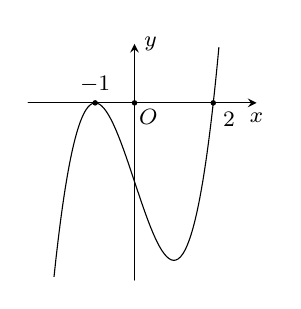
\begin{tikzpicture}[scale=1, font=\footnotesize, line join=round, line cap=round,>=stealth,x=0.5cm,y=0.5cm]
			\def \xmin{-2.7};
			\def \xmax{3.1};
			\def \ymin{-4.5};
			\def \ymax{1.5};
			\draw[->] (\xmin, 0.) -- (\xmax,0.) node[anchor=north] {$x$};
			\draw[->] (0.,\ymin) -- (0.,\ymax) node[anchor=west] {$y$};
			\clip(\xmin+0.1,\ymin+0.1) rectangle (\xmax-0.1,\ymax-0.1);
			\draw[smooth,samples=100,domain=\xmin:\xmax] plot(\x,{(\x)^3-3*(\x)-2});
			\draw[dashed] (-1,0) node[above]{$-1$} (2,0) node[below right]{$2$};
			\foreach \x/\y  in {-1/0,2/0}{\fill[black] (\x,\y) circle(1pt);}
			\foreach \x/\y/\l/\g  in {0/0/O/-45}{\fill[black] (\x,\y) circle(1pt)+(\g:0.5) node{$\l$};}
	\end{tikzpicture}}
	\loigiai{
		Từ đồ thị ta có bảng xét dấu $f'(x)$ như sau
		\begin{center}
			
\begin{tikzpicture}
				\tkzTabInit[nocadre=false, lgt=1.2, espcl=2.5, deltacl=0.6]{$x$/0.6,$f'(x)$/0.6}
				{$-\infty$, $-1$, $2$, $+\infty$}
				\tkzTabLine {,-,0,-,0,+,}
			\end{tikzpicture}
		\end{center}
		Vậy hàm số $f(x)$ có một điểm cực trị.
	}
\end{ex}

%%==========Câu 10
\begin{ex}%[Lê Hồng Phi]%[Tex hóa Đề Vted 2023]%[2D2Y6-1]
	Tập nghiệm của bất phương trình $\log_3 x<2$ là
	\choice
	{$(-\infty;9)$}
	{\True $(0;9)$}
	{$(0;6)$}
	{$(9;+\infty)$}
	\loigiai{
		Ta có $\log_3 x<2\Leftrightarrow\heva{& x>0 \\ & x<3^2}\Leftrightarrow 0<x<9$.\\
		Vậy tập nghiệm của bất phương trình đã cho là $S=(0;9)$.
	}
\end{ex}



%%Thầy Lee Van Toan
%%==========Câu 11
\begin{ex}%[Lee Van Toan]%[Tex hóa Đề Vted 2023]%[2D4Y2-1]
	Cho hai số phức $z_1=-2-3i$, $z_2=4+5i$, khi đó $z_1+z_2$ bằng
	\choice
	{$-2-2i$}
	{\True $2+2i$}
	{$-2+2i$}
	{$2-2i$}
	\loigiai{
		Ta có $z_1+z_2=(-2-3i)+(4+5i)=2+2i$.
	}
\end{ex}

%%==========Câu 12
\begin{ex}%[Lee Van Toan]%[Tex hóa Đề Vted 2023]%[1D3Y4-3]
	Cho cấp số nhân $\left(u_{n}\right)$ với $u_2=2$ và $u_3=3$. Công bội của cấp số nhân đó bằng
	\choice
	{$\dfrac{2}{3}$}
	{$1$}
	{\True $\dfrac{3}{2}$}
	{$-1$}
	\loigiai{
		Ta có $u_3=u_2 \cdot q \Rightarrow q=\dfrac{u_3}{u_2}=\dfrac{3}{2}$.
	}
\end{ex}

%%==========Câu 13
\begin{ex}%[Lee Van Toan]%[Tex hóa Đề Vted 2023]%[2D3Y1-1]
	Trên khoảng $(0;+\infty)$, họ nguyên hàm của hàm số $f(x)=\dfrac{1}{x}$ là
	\choice
	{$\ln (-x)+C$}
	{$-\ln x+C$}
	{\True $\ln x+C$}
	{$-\dfrac{1}{x^2}+C$}
	\loigiai{
		Ta có $\displaystyle\int\limits_3^5f(x) \mathrm{\,d} \dfrac{1}{x}=\ln |x|+C=\ln x+C$, với $x \in (0;+\infty)$.
	}
\end{ex}

%%==========Câu 14
\begin{ex}%[Lee Van Toan]%[Tex hóa Đề Vted 2023]%[2D1Y1-2]
	Cho hàm sô $y=f(x)$ có bảng biên thiên như sau
	\begin{center}
		
\begin{tikzpicture}
			\tkzTabInit[espcl=2.5,lgt=1.5]
			{$x$/0.7,$f'(x)$/0.7,$f(x)$/2.1}
			{$-\infty$,$-1$,$3$,$+\infty$}
			\tkzTabLine{,+,0,-,0,+,}
			\tkzTabVar{-/$-\infty$,+/$1$,-/$-3$,+/$+\infty$}
		\end{tikzpicture}
	\end{center}
	Hàm số $f(x)$ đạt cực tiểu tại điểm
	\choice
	{\True $x=3$}
	{$x=-3$}
	{$x=-1$}
	{$x=1$}
	\loigiai{
		Dựa vào bảng biến thiên ta có hàm số đạt cực tiểu tại $x=3$.	
	}
\end{ex}

%%==========Câu 15
\begin{ex}%[Lee Van Toan]%[Tex hóa Đề Vted 2023]%[2D2Y5-1]
	Nghiệm của phương trình $4^{x+1}=16$ là
	\choice
	{$x=2$}
	{$x=5$}
	{$x=-1$}
	{\True $x=1$}
	\loigiai{
		Phương trình $4^{x+1}=16 \Leftrightarrow 4^{x+1}=4^2 \Leftrightarrow x=1$.
	}
\end{ex}

%%==========Câu 16
\begin{ex}%[Lee Van Toan]%[Tex hóa Đề Vted 2023]%[2H3Y1-3]
	Trong KG $Oxyz$, mặt cầu $(S) \colon (x-1)^2+(y-2)^2+(z-3)^2=25$ có bán kính bằng
	\choice
	{$25$}
	{\True $5$}
	{$14$}
	{$225$}
	\loigiai{
		Dựa vào phương trình mặt cầu ta được có bán kính mặt cầu là $R=5$.	
	}
\end{ex}

%%==========Câu 17
\begin{ex}%[Lee Van Toan]%[Tex hóa Đề Vted 2023]%[1D2Y2-1]
	Số chỉnh hợp chập $3$ của $10$ phần tử là
	\choice
	{$\mathrm{C}_{10}^3$}
	{\True $\mathrm{A}_{10}^3$}
	{$10^3$}
	{$3^{10}$}
	\loigiai{
		Số chỉnh hợp chập $3$ của $10$ phần tử là $\mathrm{A}_{10}^3$.
	}
\end{ex}

%%==========Câu 18
\begin{ex}%[Lee Van Toan]%[Tex hóa Đề Vted 2023]%[2D2B3-2]
	Với mọi số thực dương $a$, $3^{\log _{27}a}$ bằng
	\choice
	{$3a$}
	{\True $a^3$}
	{$a^{\tfrac{1}{3}}$}
	{$\dfrac{a}{3}$}
	\loigiai{
		Với mọi số thực dương $a$, ta có $3^{\log _{27}a}=3^{3\log _3a}=\left(3^{\log_3a}\right)^3=a^3$.	
	}
\end{ex}

%%==========Câu 19
\begin{ex}%[Lee Van Toan]%[Tex hóa Đề Vted 2023]%[2D3B2-1]
	Nếu $\displaystyle\int\limits_3^5f(x) \mathrm{\,d} x=15$ thì $\displaystyle\int\limits_5^33 \cdot f(x) \mathrm{\,d} x$ bằng
	\choice
	{$45$}
	{$-5$}
	{\True $-45$}
	{$5$}
	\loigiai{
		Ta có $\displaystyle\int\limits_5^33 \cdot f(x) \mathrm{\,d} x=-3\displaystyle\int\limits_3^5 f(x) \mathrm{\,d} x=-3\cdot(15)=-45$.
	}
\end{ex}

%%==========Câu 20
\begin{ex}%[Lee Van Toan]%[Tex hóa Đề Vted 2023]%[2H3Y3-2]
	Trong KG $Oxyz$, đường thẳng $d$ qua điểm $M(-1;2;3)$ và có một véc-tơ chỉ phương $\overrightarrow{u}=(2;-1;3)$ có phương trình là
	\choice
	{$\heva{&x=-1+2t \\ &y=2-t \\ &z=3-3t}$}
	{\True $\heva{&x=-1+2t \\ &y=2-t \\ &z=3+3t}$}
	{$\heva{&x=2-t \\ &y=-1+2 t \\ &z=-3+3 t}$}
	{$\heva{&x=2+2t \\ &y=-1-t \\ &z=3+3t}$}
	\loigiai{
		Đường thẳng $d$ qua điểm $M(-1;2;3)$ và có một véc-tơ chỉ phương $\overrightarrow{u}=(2;-1;3)$ có phương trình là
		$$d \colon \heva{&x=-1+2t \\ &y=2-t \\ &z=3+3t.}$$	
	}
\end{ex}

%Thầy Loc Do
%%==========Câu 21
\begin{ex}%[Loc Do]%[Tex hóa Đề Vted 2023]%[2D2Y4-1]
	Hàm số nào dưới đây có tập xác định là khoảng $(0;+\infty)$?
	\choice
	{$y=x^{-5}$}
	{\True $y=x^{\frac{1}{5}}$}
	{$y=5^x$}
	{$y=x^5$}
	\loigiai{
		Ta có
		\begin{itemize}
			\item[•]  $y=x^{-5}$ có mũ $\alpha=-5$ nguyên âm nên hàm số xác định khi $x\neq 0$. Vậy tập xác định là $\mathbb{R}\setminus \{0\}$.
			\item[•]  $y=x^{\frac{1}{5}}$ có mũ $\alpha=\dfrac{1}{5}$ không nguyên nên hàm số xác định khi $x>0$. Vậy tập xác định là $(0;+\infty)$.
			\item[•] $y=5^x$ là hàm số mũ có tập xác định là $\mathbb{R}$.
			\item[•] $y=x^5$ có mũ $\alpha =5$ nguyên dương nên hàm số có nghĩa với mọi $x\in \mathbb{R}$, do đó tập xác định của hàm số là $\mathbb{R}$.
		\end{itemize}
	}
\end{ex}

%%==========Câu 22
\begin{ex}%[Loc Do]%[Tex hóa Đề Vted 2023]%[2D1Y5-1]
	\immini{ Hàm số nào dưới đây có đồ thị như hình vẽ bên?
		\motcot
		{$y=x^3-3x+3$}
		{$y=x^4-2x^2+3$}
		{$y=-x^3+3x+3$}
		{\True $y=-x^4+2x^2+3$}}{			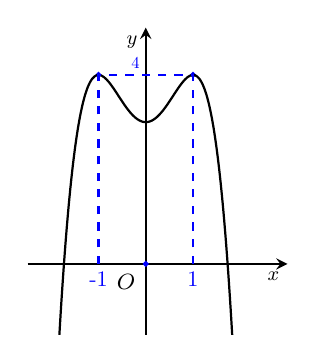
\begin{tikzpicture}[thick,>=stealth,scale=0.6] 
			\clip(-2.5,-1.5) rectangle (3,5);
			\draw[->] (-2.5,0) -- (3,0) node[below left,scale=0.8] {\small $x$};
			\draw[->] (0,-1.5) -- (0,5) node[below left,scale=0.8] {\small $y$};
			\draw [fill=black,draw=blue] (-1,4) circle (1pt);
			\draw [fill=black,draw=blue] (1,4) circle (1pt);
			\draw [fill=white,draw=blue] (0,0) circle (1pt)node[below left] {\footnotesize $O$};
			\draw[black,smooth,samples=100,domain=-2.5:2.5] plot(\x,{-(\x)^4+2*(\x)^2+3});
			\draw [dashed, blue] (1,0) node[below,scale=0.8]{1}|-(0,4)node[above left,scale=0.6]{$4$};
			\draw [dashed, blue] (-1,0) node[below,scale=0.8]{-1}|-(0,4)node[left]{};
	\end{tikzpicture}}
	\loigiai{
		\begin{itemize}
			\item[•]Hình vẽ bên có dạng đồ thị hàm bậc bốn $y=ax^4+bx^2+c$ nên loại $y=x^3-3x+3$ và $y=-x^3+3x+3$.
			\item[•] Ta có $\lim \limits_{x\to +\infty} y=-\infty$  nên $a<0$ chọn $y=-x^4+2x^2+3$.
		\end{itemize}
	}
\end{ex}

%%==========Câu 23
\begin{ex}%[Loc Do]%[Tex hóa Đề Vted 2023]%[2H1Y3-2]
	Thể tích của khối lập phương bằng $64$ thì độ dài cạnh khối lập phương đó bằng
	\choice
	{$4\sqrt{2}$}
	{\True $4$}
	{$32$}
	{$8$}
	\loigiai{
		\immini{
			Thể tích khối lập phương cạnh $a$ là
			\[
			V=a^3 =64 \Leftrightarrow a=\sqrt[3]{64}=4.
			\]
		}{
			\begin{tikzpicture}[line join=round,line cap=round,line width=.6pt,font=\footnotesize,scale=1]
				\coordinate[label=below left:$B$] (B) at (0,0);
				\coordinate[label=above left:$A$] (A) at (1,.5);
				\coordinate[label=below right:$C$] (C) at (2.5,0);
				\coordinate[label=above right:$D$] (D) at ($(C)-(B)+(A)$);
				\coordinate[label=above left:$A'$] (A1) at ($(A)+(90:2.5)$);
				\coordinate[label=left:$B'$] (B1) at ($(B)-(A)+(A1)$);
				\coordinate[label=below right:$C'$] (C1) at ($(C)-(A)+(A1)$);
				\coordinate[label=above right:$D'$] (D1) at ($(D)-(A)+(A1)$);
				\draw (B1)--(B)--(C)--(D)--(D1)--(A1)--(B1)--(C1)--(D1) (C)--(C1);
				\draw[dashed] (A)--(D) (A1)--(A)--(B);
				%\fill (A)circle(2pt) (B)circle(2pt) (C)circle(2pt) (D)circle(2pt) (A1)circle(2pt) (B1)circle(2pt) (C1)circle(2pt) (D1)circle(2pt);
			\end{tikzpicture}
		}
	}
\end{ex}

%%==========Câu 24
\begin{ex}%[Loc Do]%[Tex hóa Đề Vted 2023]%[2D4Y1-1]
	Mô-đun của số phức $z=5-3i$ bằng
	\choice
	{$8$}
	{\True $\sqrt{34}$}
	{$2\sqrt{2}$}
	{$34$}
	\loigiai{
		Ta có $|z| =|5-3i|= \sqrt{5^2+(-3)^2}=\sqrt{34}$.
	}
\end{ex}

%%==========Câu 25
\begin{ex}%[Loc Do]%[Tex hóa Đề Vted 2023]%[2D3B2-1]
	Nếu $\displaystyle \int\limits_2^3 f(x) \mathrm{\,d}x=4$ thì $\displaystyle \int\limits_2^3 \left[2-f(x)\right]\mathrm{\,d}x$ bằng
	\choice
	{\True $-2$}
	{$6$}
	{$2$}
	{$-6$}
	\loigiai{
		Ta có
		\[
		\displaystyle \int\limits_2^3 \left[2-f(x)\right]\mathrm{\,d}x
		=\displaystyle \int\limits_2^3 2\mathrm{\,d}x-\int\limits_2^3 f(x)\mathrm{\,d}x
		=2x\bigg|_2^3-\displaystyle \int\limits_2^3 f(x)\mathrm{\,d}x
		=2(3-2)-4=-2.
		\]
	}
\end{ex}

%%==========Câu 26
\begin{ex}%[Loc Do]%[Tex hóa Đề Vted 2023]%[2D3B1-1]
	Họ nguyên hàm của hàm số $f(x)=2x+\sin 4x$ là
	\choice
	{$x^2+\dfrac{1}{4}\cos 4x+C$}
	{$x^2+4\cos 4x+C$}
	{\True $x^2-\dfrac{1}{4}\cos 4x+C$}
	{$x^2-4\cos 4x+C$}
	\loigiai{
		Ta có 
		\[
		\displaystyle\int f(x)\mathrm{\,d}x=\displaystyle \int \left(2x+\sin 4x\right)\mathrm{\,d}x
		=x^2-\dfrac{1}{4}\cos 4x+C.
		\]
	}
\end{ex}

%%==========Câu 27
\begin{ex}%[Loc Do]%[Tex hóa Đề Vted 2023]%[2D4B3-2]
	Cho số phức $z$ thỏa mãn $(1+i)(2z-\overline{z})=8-4i$. Số phức $\overline{z}$ là
	\choice
	{$2-6i$}
	{\True $2+2i$}
	{$2+6i$}
	{$2-2i$}
	\loigiai{
		Giả sử $z=a+bi \Rightarrow \overline{z}=a-bi, a,b\in \mathbb{R}$. Ta có
		\begin{eqnarray*}
			& & (1+i)(2z-\overline{z})=8-4i\\
			&\Leftrightarrow &(1+i)\left(2(a+bi)-(a-bi)\right)=8-4i \Leftrightarrow (1+i)(a+3bi)=8-4i\\
			&\Leftrightarrow & (a-3b)+(a+3b)i=8-4i \Leftrightarrow 
			\heva{
				&a-3b=8\\
				&a+3b=-4
			}\Leftrightarrow \heva{
				&a=2\\
				&b=-2.
			}
		\end{eqnarray*}
		Vậy $z=2-2i \Rightarrow \overline{z}=2+2i$.
	}
\end{ex}

%%==========Câu 28
\begin{ex}%[Loc Do]%[Tex hóa Đề Vted 2023]%[2H3B2-3]
	Trong KG $Oxyz$, mặt phẳng $(\alpha)$ đi qua $A(2;-2;-1)$ và song song với mặt phẳng $(\beta):x-y+2z+5=0$ có phương trình là
	\choice
	{$x-y+2z+2=0$}
	{$x-y-2z-6=0$}
	{\True $x-y+2z-2=0$}
	{$-x+y+2z-2=0$}
	\loigiai{
		Ta có $(\alpha):\heva{
			&\text{đi qua } A(2;-2;-1)\\
			&(\alpha) \parallel (\beta) \Rightarrow \overrightarrow{n}_{(\alpha)}=\overrightarrow{n}_{(\beta)}=(1;-1;2).
		}$\\
		Phương trình mặt phẳng $(\alpha)$ là
		\[
		1(x-2)-1(y+2)+2(z+1)=0
		\Leftrightarrow x-y+2z-2=0.
		\]
	}
\end{ex}

%%==========Câu 29
\begin{ex}%[Loc Do]%[Tex hóa Đề Vted 2023]%[2D2Y4-2]
	Đạo hàm của hàm số $y=8^x$ là
	\choice
	{$y'=\dfrac{8^x}{\ln 8}$}
	{\True $y'=8^x\ln 8$}
	{$y'=x8^x\ln 8$}
	{$x8^{x-1}$}
	\loigiai{
		Áp dụng công thức $(a^x)'=a^x\ln a$. Ta có $y'= \left(8^x\right)' =8^x\ln 8$.
	}
\end{ex}

%%==========Câu 30
\begin{ex}%[Loc Do]%[Tex hóa Đề Vted 2023]%[2D3B2-2]
	Xét $I=\displaystyle \int\limits_0^{\frac{\pi}{2}}\cos^7 x\sin x\mathrm{\,d}x$ bằng cách đặt $t=\cos x$, mệnh đề nào dưới đây đúng?
	\choice
	{$I=\displaystyle \int\limits_0^{\frac{\pi}{2}} t^7 \mathrm{\,d}t$}
	{$I=-\displaystyle \int\limits_0^{\frac{\pi}{2}} t^7 \mathrm{\,d}t$}
	{\True $I=\displaystyle \int\limits_0^1  t^7 \mathrm{\,d}t$}
	{$I=-\displaystyle \int\limits_0^1 t^7 \mathrm{\,d}t$}
	\loigiai{
		Đặt $t=\cos x \Rightarrow  \mathrm{\,d}t =-\sin x  \mathrm{\,d}x \Rightarrow \sin x  \mathrm{d}x=- \mathrm{\,d}t$.\\
		Đổi cận: $x=0 \Rightarrow t=1; x=\dfrac{\pi}{2}\Rightarrow t=0$.\\
		Khi đó 
		\[
		I=\displaystyle \int\limits_1^0 t^7 (-\mathrm{\,d}t) =\displaystyle \int\limits_0^1 t^7 \mathrm{\,d}t.
		\]
	}
\end{ex}


%Cô Lương Như Quỳnh
%%==========Câu 31
\begin{ex}%[Lương Như Quỳnh]%[Tex hóa Đề Vted 2023]%[2D1B5-4]
	Tọa độ giao điểm của đồ thị hàm số $ y=x^3-3x^2+2 $ với trục tung là 
	\choice
	{\True $(0;2)$}
	{$(0;-2)$}
	{$(1;0)$}
	{$(-1;0)$}
	\loigiai{
		Xét hàm số $ y=x^3-3x^2+2$. Ta có $ x=0\Rightarrow y=2 $.\\
		Vậy tọa độ giao điểm của đồ thị hàm số đã cho với trục tung là $(0;2)$.
	}
\end{ex}

%%==========Câu 32
\begin{ex}%[Lương Như Quỳnh]%[Tex hóa Đề Vted 2023]%[2D1B3-1]
	Cho hàm số $ f(x) $ có đạo hàm $ f'(x)=(x-1)(x-2)(x+4)^2 $, $ \forall x\in \mathbb{R} $. Trên đoạn $ [-4;2] $, hàm số $ f(x) $ đạt giá trị lớn nhất tại điểm 
	\choice
	{$x=-4$}
	{\True $x=1$}
	{$x=2$}
	{$x=-2$}
	\loigiai{
		Ta có $ f'(x)=0\Leftrightarrow \hoac{&x=1\\&x=2\\&x=-4.} $
		\begin{center}
			
\begin{tikzpicture}
				\tkzTabInit[nocadre=false,lgt=1.2,espcl=2.5,deltacl=0.6]
				{$x$ /0.6, $f'(x)$ /0.6, $f(x)$ /2.}
				{$-4$,$1$,$2$}
				\tkzTabLine{$0$,+,$0$,-,$0$}
				\tkzTabVar{-/$ $,+/$ $,-/$ $}
			\end{tikzpicture}
		\end{center}
		Vậy trên đoạn $ [-4;2] $, hàm số $ f(x) $ đạt giá trị lớn nhất tại điểm $ x=1 $.
	}
\end{ex}

%%==========Câu 33
\begin{ex}%[Lương Như Quỳnh]%[Tex hóa Đề Vted 2023]%[2D2B3-2]
	Với mọi số thực dương $a$, $b$ thỏa mãn $\log_3a+2\log_3b=2$, khẳng định nào dưới đây đúng?
	\choice
	{$ab^2=6$}
	{$a+b^2=9$}
	{$a+b^2=6$}
	{\True $ab^2=9$}
	\loigiai{
		Với mọi số thực dương $a$, $b$, ta có $\log_3a+2\log_3b=2 \Leftrightarrow \log_3\left(ab^2\right)=2\Leftrightarrow ab^2=9$.
	}
\end{ex}

%%==========Câu 34
\begin{ex}%[Lương Như Quỳnh]%[Tex hóa Đề Vted 2023]%[2H1B3-4]
	\immini{Cho hình lăng trụ đứng $ABC.A'B'C'$ có đáy $ ABC $ là tam giác vuông cân tại $ A $ và \break$ AB=AA'=4 $ (tham khảo hình bên). Góc giữa hai đường thẳng $ A'B $ và $ B'C' $ bằng 
		\choice
		{$90^\circ$}
		{$30^\circ$}
		{$45^\circ$}
		{\True $60^\circ$}}
	{
		\begin{tikzpicture}[scale=0.6, font=\footnotesize, line join=round, line cap=round, >=stealth]
			\def\ac{4} % cạnh AC
			\def\ab{2} % cạnh AB
			\def\h{4} % chiều cao
			\def\gocA{50} % góc A của đáy
			\coordinate[label=left:$A$] (A) at (0,0);
			\coordinate[label=right:$C$] (C) at (\ac,0);
			\coordinate[label=below left:$B$] (B) at (-\gocA:\ab);
			\coordinate[label=left:$A'$] (A') at ($(A)+(90:\h)$);
			\coordinate[label=below right:$B'$] (B') at ($(B)-(A)+(A')$);
			\coordinate[label=right:$C'$] (C') at ($(C)-(A)+(A')$);
			
			\draw (A')--(A)--(B)--(C)--(C')--(A')--(B')--(C') (B)--(B');
			\draw[dashed] (A)--(C);
			\foreach \diem in {A,B,C,A',B',C'} \fill (\diem)circle(1.5pt);
		\end{tikzpicture}
	}
	\loigiai{
		\immini{
			Vì $ B'C'\parallel BC $ nên $ (A'B,B'C')=(A'B,BC) $.\\
			Ta có $ \triangle A'AB=\triangle A'AC $ (c-g-c) suy ra $ A'B=A'C $. Do đó $ \triangle BA'C $ cân tại $ A' $.\\
			Gọi $ M $ là trung điểm $ BC $ suy ra $ A'M\perp BC $.\\
			Xét tam giác $ A'AB $ vuông cân tại $A$ có $ AB=AA'=4 \Rightarrow A'B=4\sqrt{2} $.\\
			Xét tam giác $ ABC $ vuông cân tại $A$ có $ AB=AC=4 \Rightarrow BC=4\sqrt{2} $.\\
			Suy ra tam giác $ A'BC $ đều. Do đó $(A'B,BC)=\widehat{A'BC}=60^\circ $.\\
		}
		{
			\begin{tikzpicture}[scale=0.6, font=\footnotesize, line join=round, line cap=round, >=stealth]
				\def\ac{4} % cạnh AC
				\def\ab{2} % cạnh AB
				\def\h{4} % chiều cao
				\def\gocA{50} % góc A của đáy
				\coordinate[label=left:$A$] (A) at (0,0);
				\coordinate[label=right:$C$] (C) at (\ac,0);
				\coordinate[label=below left:$B$] (B) at (-\gocA:\ab);
				\coordinate[label=left:$A'$] (A') at ($(A)+(90:\h)$);
				\coordinate[label=below right:$B'$] (B') at ($(B)-(A)+(A')$);
				\coordinate[label=right:$C'$] (C') at ($(C)-(A)+(A')$);
				\coordinate[label=below right:$M$] (M) at ($(B)!1/2!(C)$);
				\draw (A')--(A)--(B)--(C)--(C')--(A')--(B')--(C') (A')--(B)--(B');
				\draw[dashed] (A)--(C)--(A')--(M);
				\foreach \diem in {A,B,C,A',B',C',M} \fill (\diem)circle(1.5pt);
			\end{tikzpicture}
		}
	}
\end{ex}

%%==========Câu 35
\begin{ex}%[Lương Như Quỳnh]%[Tex hóa Đề Vted 2023]%[2H2K2-6]
	Một cái cốc nước hình trụ có chiều cao bằng $12$ cm, bán kính đáy bằng $3$ cm. Người ta đổ vào cốc một lượng nước sao cho chiều cao mực nước là $4$ cm (so với đáy cốc), sau đó bỏ vào cốc một quả cầu kim loại có bán kính bằng $2$ cm thì chiều cao mực nước trong cốc tăng thêm bao nhiêu cm? (giả sử độ dày đáy và thành cốc không đáng kể)
	\choice
	{\True $1{,}19$ cm}
	{$5{,}19$ cm}
	{$5{,}77$ cm}
	{$2{,}77$ cm}
	\loigiai{
		Thể tích nước trong cốc là $ V_{\text{nước}}=\pi R_{\text{trụ}}^2\cdot h=\pi \cdot 3^2\cdot 4= 36\pi$ cm$ ^3 $.\\
		Thể tích quả cầu là $ V_{\text{cầu}}=\dfrac{4}{3}\pi R_{\text{cầu}}^3=\dfrac{4}{3}\pi \cdot 2^3\approx 10{,}67 \pi $ cm$ ^3 $.\\
		Thể tích nước và quả cầu là $ V=V_{\text{nước}}+V_{\text{cầu}}=36\pi +10{,}67\pi =46{,}67\pi $ cm$ ^3 $.\\
		Gọi $ x $ cm là chiều cao mực nước trong cốc sau khi bỏ một quả cầu vào cốc. Ta có 
		\[V=\pi R^2\cdot x \Rightarrow x=\dfrac{V}{\pi R^2}=\dfrac{46{,}67\pi}{\pi \cdot 3^2} =5{,}19.\]
		Vậy chiều cao mực nước trong cốc tăng thêm là $ 5{,}19-4=1{,}19 $ cm.
	}
\end{ex}

%%==========Câu 36
\begin{ex}%[Lương Như Quỳnh]%[Tex hóa Đề Vted 2023]%[1H3B5-3]
	\immini{Hình chóp $ S. ABC $ có đáy $ABC$ vuông tại $B$, tam giác $ SAB $ vuông tại $B$, tam giác $ SBC $ vuông tại $S$. Biết $AB=a$, $SA=2a$, $BC=4a$ (tham khảo hình vẽ). Khoảng cách từ $C$ đến mặt phẳng $(SAB)$ bằng
		\choice
		{\True $\sqrt{13}a$}
		{$\sqrt{15}a$}
		{$4a$}
		{$\sqrt{11}a$}}
	{
		\begin{tikzpicture}[scale=0.6, font=\footnotesize, line join=round, line cap=round, >=stealth]
			\def\ac{4} % cạnh AC
			\def\ab{2} % cạnh AB
			\def\h{4} % chiều cao
			\def\gocA{50} % góc A của đáy
			\coordinate[label=left:$A$] (A) at (0,0);
			\coordinate[label=right:$C$] (C) at (\ac,0);
			\coordinate[label=below left:$B$] (B) at (-\gocA:\ab);
			\coordinate[label=left:$S$] (S) at ($(A)+(60:\h)$);
			\draw (S)--(A)--(B)--(C)--cycle (S)--(B);
			\draw[dashed] (A)--(C);
			\foreach \x/\y/\z in {A/B/C,B/S/C}{
				\path pic[draw,angle radius=5pt]{right angle= \x--\y--\z};
			}
				\path pic[draw,angle radius=8pt]{right angle= A--B--S};
			\foreach \diem in {A,B,C,S} \fill (\diem)circle(1.5pt);
		\end{tikzpicture}
	}
	\loigiai{
		Ta có $ \heva{&AB\perp BC\\&AB\perp BS} $ suy ra $  AB\perp (SBC) \Rightarrow AB\perp SC$. Mà $ SC\perp SB $ nên $ SC\perp (SAB) $.\\
		Do đó $ \mathrm{d}(C,(SAB)) =SC$.\\
		Xét tam giác $ SBC $ vuông tại $ S $ có $ SC=\sqrt{BC^2-SB^2}=\sqrt{BC^2-\left(SA^2-AB^2\right)} =\sqrt{(4a)^2-\left((2a)^2-a^2\right)}=\sqrt{13}a$.
	}
\end{ex}

%%==========Câu 37
\begin{ex}%[Lương Như Quỳnh]%[Tex hóa Đề Vted 2023]%[1D2K5-5]
	Chọn ngẫu nhiên hai số trong $40$ số nguyên dương đầu tiên. Tính xác suất để hai số được chọn có tổng là một số chia hết cho $3$.
	\choice
	{$\dfrac{1}{10}$}
	{$\dfrac{13}{60}$}
	{\True $\dfrac{1}{3}$}
	{$\dfrac{7}{30}$}
	\loigiai{
		Số cách chọn ngẫu nhiên là $ \mathrm{C}_{40}^2 $. Với $ 40 $ số nguyên dương đầu tiên chia thành $ 3 $ nhóm:
		\begin{itemize}
			\item Nhóm $ (1) $ chia hết cho $ 3 $ là các số $ 3;6;\ldots ;39 $ gồm $ 13 $ số.
			\item Nhóm $ (2) $ chia cho $ 3 $ dư $ 1 $ là các số $ 1;4;\ldots ;40 $ gồm $ 14 $ số.
			\item Nhóm $ (3) $ chia cho $ 3 $ dư $ 2 $ là các số $ 2;5;\ldots ;38 $ gồm $ 13 $ số.
		\end{itemize}
		Để tổng hai số là một số chia hết cho $ 3 $ có các khả năng sau: cả hai số thuộc nhóm $ (1) $; hoặc một số thuộc nhóm $ (2) $ và một số thuộc nhóm $ (3) $.\\
		Xác suất cần tính là $ \mathrm{P}=\dfrac{ \mathrm{C}_{13}^2 + \mathrm{C}_{14}^1\cdot \mathrm{C}_{13}^1}{\mathrm{C}_{40}^2}=\dfrac{1}{3}$.
	}
\end{ex}

%%==========Câu 38
\begin{ex}%[Lương Như Quỳnh]%[Tex hóa Đề Vted 2023]%[2H3K3-8]
	Trong KG $Oxyz$, cho đường thẳng $ \Delta \colon \dfrac{x-1}{-1}=\dfrac{y}{2}=\dfrac{z+1}{1} $ và mặt phẳng $ (\alpha) \colon x+2y-2z-1=0 $. Biết mặt phẳng $ (P) $ chứa $ \Delta $ và tạo với $(\alpha)$ một góc nhỏ nhất có phương trình dạng $ 7x+by+cz+d=0 $. Giá trị $ b+c+d $ là 
	\choice
	{$-3$}
	{\True $-23$}
	{$3$}
	{$-5$}
	\loigiai{
		Ta có $A(1;0;-1) \in \Delta$; một véc-tơ chỉ phương của đường thẳng $ \Delta $ là $\overrightarrow{u}_{\Delta}=(-1;2;1)$; một véc-tơ pháp tuyến của mặt phẳng $ (P) $ là $ \overrightarrow{n}_P=(7 ; b;c) $.\\
		Vì $\Delta \subset(P) $ nên $ \heva{&A(1;0;-1) \in(P) \\ &\overrightarrow{u}_{\Delta} \perp \overrightarrow{n}_P} \Leftrightarrow \heva{&7-c+d=0 \\ &-7+2 b+c=0} \Leftrightarrow \heva{&c=7-2 b \\ &d=-2 b} \Rightarrow \overrightarrow{n}_P=(7;b;7-2b)$.\\
		Khi đó $\cos ((P),(\alpha))=g(b)=\dfrac{|7+2 b-2(7-2 b)|}{3 \sqrt{49+b^2+(7-2 b)^2}} \leq \max \limits_{\mathbb{R}} g(b)=g(10)=\dfrac{\sqrt{318}}{18} $.\\
		Suy ra $((P),(\alpha)) \geq \arccos \dfrac{\sqrt{318}}{18}$.\\
		Dấu \lq\lq =\rq\rq\, xảy ra khi và chỉ khi $b=10 \Rightarrow c=-13 $; $d=-20 \Rightarrow b+c+d=-23$.
	}
\end{ex}

%%==========Câu 39
\begin{ex}%[Lương Như Quỳnh]%[Tex hóa Đề Vted 2023]%[2D4K2-3]
	Trên tập số phức, xét phương trình $ z^2+az+b=0 $ ($a$, $b\in \mathbb{R}$). Có bao nhiêu cặp số $ (a;b) $ để phương trình đã cho có hai nghiệm là $ z_1=3m-2-\left(m^3+m^2\right) \cdot i$ và $ z_2=m^3+2m\cdot i $ (với $ m $ là tham số thực)?
	\choice
	{$2$}
	{$4$}
	{$1$}
	{\True $3$}
	\loigiai{
		{\bf TH1.} Nếu $z_1$, $z_2 \in \mathbb{R} $ thì $ \heva{
			&m^3+m^2=0 \\&2 m=0} \Leftrightarrow m=0 \Rightarrow \heva{&z _1= - 2 \\&z_ 2= 0} \Rightarrow \heva{&a=-\left(z_1+z_2\right)=2 \\&b=z_1 z_2=0.}$\\
		{\bf TH2.} Nếu $z_1$, $z_2 \notin \mathbb{R} $ thì $ z_2=\overline{z}_1 \Leftrightarrow \heva{ 
			&m^3= 3m - 2\\&2 m = m^3+ m^2 } \Leftrightarrow \hoac{&m=1 \\&m=-2.}$\\
		Khi $m=1 \Rightarrow z_1=1-2 i$; $z_2=1+2 i \Rightarrow \heva{
			&a=-\left(z_1+z_2\right)=-2 \\&b=z_1 z_2=5.}$\\
		Khi $m=-2 \Rightarrow z_1=-8+4 i$; $z_2=-8-4 i \Rightarrow \heva{
			&a=-\left(z_1+z_2\right)=16 \\
			&b=z_1 z_2=80.}$\\
		Vậy có $3$ cặp số $(a ; b)$ thỏa mãn.
	}
\end{ex}

%%==========Câu 40
\begin{ex}%[Lương Như Quỳnh]%[Tex hóa Đề Vted 2023]%[2H2K1-2]
	Cho một hình nón đỉnh $S$ có độ dài đường sinh bằng $10 $ cm, bán kính đáy bằng $6$ cm. Cắt hình nón đã cho bởi mặt phẳng song song với đáy của nón thu được một hình nón $(N)$ đỉnh $S$ có chiều cao bằng $\dfrac{16}{5}$ cm. Diện tích xung quanh của $(N)$ bằng
	\choice
	{$\dfrac{192 \pi}{25}$ cm$^2$}
	{\True $\dfrac{48 \pi}{5}$ cm$^2$}
	{$\dfrac{768 \sqrt{34} \pi}{625}$ cm$^2$}
	{$\dfrac{768 \pi}{25}$ cm$^2$}
	\loigiai{
		\immini{
			Hình nón ban đầu có $r=6 $ cm; $\ell=10 $ cm; $h=\sqrt{\ell^2-r^2}=8$ cm.\\
			Gọi $r_1$, $h_1$, $\ell_1$ lần lượt là bán kính đáy, chiều cao và độ dài đường sinh của $(N)$.\\
			Theo Ta-lét có $\dfrac{r_1}{r}=\dfrac{h_1}{h} \Leftrightarrow r_1=\dfrac{h_1}{h} \cdot r=\dfrac{\dfrac{16}{5}}{8} \cdot 6=\dfrac{12}{5}$ cm.\\
			Do đó $\ell_1=\sqrt{r_1^2+h_1^2}=\sqrt{\left(\dfrac{12}{5}\right)^2+\left(\dfrac{16}{5}\right)^2}=4\text{cm} \Rightarrow S_{\text{xq}}=\pi r_1 \ell_1=\pi \cdot \dfrac{12}{5} \cdot 4=\dfrac{48 \pi}{5}$ cm$ ^2 $.
		}
		{
			\begin{tikzpicture}[scale=0.6, font=\footnotesize, line join=round, line cap=round, >=stealth]
				\def\ac{4} % cạnh AC
				\def\h{5} % cạnh AB
				\coordinate[label=left:$A$] (A) at (0,0);
				\coordinate[label=right:$B$] (B) at (\ac,0);
				\coordinate[label=above left:$O$] (O) at ($(A)!1/2!(C)$);
				\coordinate[label=left:$S$] (S) at ($(O)+(90:\h)$);
				\coordinate[label=above left:$A_1$] (A_1) at ($(A)!1/2!(S)$);
				\coordinate[label=above right:$B_1$] (B_1) at ($(B)!1/2!(S)$);
				\coordinate[label=below left:$O_1$] (O_1) at ($(A_1)!1/2!(B_1)$);
				\draw (A)--(S)--(B)--cycle (A_1)--(B_1) (S)--(O);
				\foreach \diem in {A,S,B,A_1,B_1,O_1,O} \fill (\diem)circle(1.5pt);
				\node at (2.5,2.5) [above]{$r_1$};
				\node at (2.2,3.5) [left]{$h_1$};
				\node at (3,0) [above]{$r$};
			\end{tikzpicture}
	}}
\end{ex}



%Thầy Nguyen Chien Thang
%%==========Câu 41
\begin{ex}%[Nguyen Chien Thang]%[Tex hóa Đề Vted 2023]%[2D1G3-1]
	Cho hàm số $f(x)=\dfrac{m x-6 \sqrt{x+2}}{x+3},(m \in \mathbb{R})$. Có bao nhiêu giá trị nguyên của $m$ để $\mathop {\min }\limits_{[ 2;7 ]}|f(x)|\leq 1 ?$
	\choice
	{$1$}
	{\True $7$}
	{$2$}
	{$6$}
	\loigiai{ 
		Ta có
		$$
		\begin{aligned}
			&\mathop {\min }\limits_{[ 2;7 ]}|f(x)| \leq 1 \Leftrightarrow\left|\dfrac{m x-6 \sqrt{x+2}}{x+3}\right| \leq 1 \text { có nghiệm } x \in[2 ; 7]  \\
			& \Leftrightarrow-1 \leq \dfrac{m x-6 \sqrt{x+2}}{x+3} \leq 1 \text { có nghiệm } x \in[2 ; 7]  \\
			& \Leftrightarrow g(x)=\dfrac{-x-3+6 \sqrt{x+2}}{x} \leq m \leq h(x)=\dfrac{x+3+6 \sqrt{x+2}}{x} \text { có nghiệm } x \in[2 ; 7]  \\ 
			& \Leftrightarrow \min_{[2 ; 7]}g(x)=g(7)=\dfrac 87 \leq m \leq \max _{[2 ; 7]} h(x)=h(2)=\dfrac{17}{2} \Rightarrow m \in\{2, \ldots, 8\} .
		\end{aligned}
		$$
		
	}
\end{ex}

%%==========Câu 42
\begin{ex}%[Nguyen Chien Thang]%[Tex hóa Đề Vted 2023]%[2D2G6-5]
	Có bao nhiêu số nguyên dương $b$ sao cho ứng với mỗi $b$ có không quá $31$ số nguyên $a$ thoả mãn $$\log_{4b}\left(\dfrac{a^3}{2^{10}b^2}\right)\leq\log_a\dfrac b{16}?$$
	\choice
	{\True $8$}
	{$4$}
	{$5$}
	{$7$}
	\loigiai{
		Với số nguyên dương $b$ điều kiện của bẩt phương trình là $0<a \neq 1$, kết hợp với xét $a$ nguyên nên $a \geq 2$.\\
		Đổi Cơ Số logarit về cơ số $2$ ta được $$\log_{4b}\left(\dfrac{a^3}{2^{10}b^2}\right)\leq\log_a\dfrac b{16}\Leftrightarrow\dfrac{3\log_2a-10-2\log_2b}{2+\log_2b}\leq\dfrac{\log_2b-4}{\log_2a}.$$
		Đặt $x=\log _2 a ; y=\log _2 b,(x, y>0)$.\\
		Suy ra $ \dfrac{3 x-10-2 y}{y+2} \leq \dfrac{y-4}{x} \Leftrightarrow(y+2)(y-4) \geq x(3 x-10-2 y)$
		$\Leftrightarrow 3 x^2-(2 y+10) x-(y+2)(y-4) \leq 0$ có hai nghiệm đối với $x$ là $y+2 ; \dfrac{4-y}{3}$ và $y+2>\dfrac{4-y}{3}, \forall y>0$.\\
		Do đó $$\dfrac{4-y}3\leq x\leq y+2\Leftrightarrow\log_2\sqrt[3]{\dfrac{16}b}\leq\log_2a\leq\log_2(4b)\Leftrightarrow\sqrt[3]{\dfrac{16}b}\leq a\leq 4b
		\Rightarrow S_a=\left[\sqrt[3]{\dfrac{16}b}; 4b\right]$$ chứa tối đa $31$ số nguyên là các số $4 b, 4 b-1, \ldots, 4 b-30 \Leftrightarrow 4 b-31<\sqrt[3]{\dfrac{16}{b}} \Rightarrow b \in\{1, \ldots, 8\}$.
		
	}
\end{ex}

%%==========Câu 43
\begin{ex}%[Nguyen Chien Thang]%[Tex hóa Đề Vted 2023]%[2H1B3-2]
	Cho khối lăng trụ tam giác đều $ABC.A'B'C'$ có cạnh bên bằng $2a$, góc giữa hai mặt phẳng $\left(A' B C\right)$ và $\left(A B' C'\right)$ bằng $90^\circ$. Thể tích của khối lăng trụ đã cho bằng
	\choice
	{$2 \sqrt{3} a^3$}
	{\True $\dfrac{8 \sqrt{3}}{3} a^3$}
	{$\dfrac{2 \sqrt{3}}{3} a^3$}
	{$\dfrac{8 \sqrt{3}}{9} a^3$}
	\loigiai{
		Ta có $\left(A' B C\right) \cap\left(A B' C'\right)=P Q \parallel B C \parallel B' C'$.\\ Gọi $M, N$ lần lượt là trung điểm $B C, B' C'$ khi đó $\left(A M N A'\right) \perp B C \parallel B' C' \parallel P Q$.
		\begin{center}
			\begin{tikzpicture}[scale=1, font=\footnotesize, line join=round, line cap=round, >=stealth]
				\def\ac{4} % cạnh AC
				\def\ab{2} % cạnh AB
				\def\h{4} % chiều cao
				\def\gocA{50} % góc A của đáy
				\coordinate[label=left:$A$] (A) at (0,0);
				\coordinate[label=right:$C$] (C) at (\ac,0);
				\coordinate[label=below left:$B$] (B) at (-\gocA:\ab);
				\coordinate[label=left:$A'$] (A') at ($(A)+(90:\h)$);
				\coordinate[label=below left:$B'$] (B') at ($(B)-(A)+(A')$);
				\coordinate[label=right:$C'$] (C') at ($(C)-(A)+(A')$);
				\coordinate[label=below:$M$] (M) at ($(C)!0.5!(B)$);
				\coordinate[label=above:$N$] (N) at ($(C')!0.5!(B')$);
				\coordinate[label=left:$P$] (P) at ($(A')!0.5!(B)$);
				\coordinate[label=right:$Q$] (Q) at ($(A')!0.5!(C)$);
				\coordinate (H) at (intersection cs:first line={(A)--(N)},second line={(P)--(Q)});
				
				\draw (A')--(A)--(B)--(C)--(C')--(A')--(B')--(C') (B)--(B')--(A) (B)--(A')--(N)--(M);
				\draw[dashed] (M)--(A)--(C) (A')--(C) (N)--(A)--(C') (P)--(Q);
				\foreach \diem in {A,B,C,A',B',C',M,N,P,Q,H} \fill (\diem)circle(1.5pt);
			\end{tikzpicture}	
		\end{center}
		Nên $\widehat{\left(\left(A' B C\right),\left(A B' C'\right)\right)}=\widehat{\left(A N, A' M\right)}=90^\circ \Rightarrow A M N A'$ là hình vuông nên $$A M=A A'=2a\Rightarrow B C=\dfrac 2{\sqrt 3}A M=\dfrac 4{\sqrt 3}a.$$
		
		Vậy $V_{A B C \cdot A' B' C'}=S_{A B C} \cdot A A'=\dfrac{\sqrt{3}}{4}\left(\dfrac{4 a}{\sqrt{3}}\right)^2 2 a=\dfrac{8 \sqrt{3}}{3} a^3$.
		
	}
\end{ex}

%%==========Câu 44
\begin{ex}%[Nguyen Chien Thang]%[Tex hóa Đề Vted 2023]%[2D1G5-3]
	Cho hàm số bậc ba $f(x)$ có đồ thị như hình vẽ:
	
	\begin{center}
		\begin{tikzpicture}[line cap=butt,line join=miter,>=stealth]
			\tikzset{declare function={xmin=-2;xmax=4;ymin=-2;ymax=4;
					f(\x)=0.5*(\x)^3-1.5*(\x)^2+2;
				},
				smooth,samples=450
			}
			\draw[->] (xmin,0)--(xmax,0) node[shift={(-100:7pt)},font=\normalsize]{$ x $};
			\draw[->] (0,ymin)--(0,ymax) node[shift={(190:7pt)},font=\normalsize]{$ y $};
			\fill (0,0) node[shift={(225:7pt)},font=\normalsize]{$ O $};
			\draw (-1,0)node[below left]{$-1$} (2,0)node[below]{$2$}  (0,2)node[above left]{$2$} 
			;
			\fill (-1,0) circle (1pt); \fill (2,0) circle (1pt); \fill (0,2) circle (1pt);
			\clip (xmin,ymin) rectangle (xmax,ymax);
			\draw  plot[domain=xmin:xmax] (\x, {f(\x)});
		\end{tikzpicture}
	\end{center}
	
	Số nghiệm thực phân biệt của phương trình $f'(x \cdot f(x))=0$ là
	
	\choice
	{$3$}
	{$4$}
	{\True $5$}
	{$2$}
	\loigiai{
		Ta có $f'(x)=0 \Leftrightarrow x=0 ; x=2$. Do đó $$f'(x \cdot f(x))=0 \Leftrightarrow\hoac{&x \cdot f(x)=0  \\&  x \cdot f(x)=2} \Leftrightarrow\hoac{&x=0 ; x=-1 ; x=2  \\&  f(x)=\dfrac{2}{x} \Rightarrow \text{có hai nghiệm}.}$$
		\begin{center}
			\begin{tikzpicture}[line cap=butt,line join=miter,>=stealth]
				\tikzset{declare function={xmin=-3;xmax=4;ymin=-2;ymax=4;
						f(\x)=0.5*(\x)^3-1.5*(\x)^2+2;g(\x)=(0*(\x)+2)/((\x)+0);
					},
					smooth,samples=450
				}
				\draw[->] (xmin,0)--(xmax,0) node[shift={(-100:7pt)},font=\normalsize]{$ x $};
				\draw[->] (0,ymin)--(0,ymax) node[shift={(190:7pt)},font=\normalsize]{$ y $};
				\fill (0,0) node[shift={(225:7pt)},font=\normalsize]{$ O $};
				\draw (-1,0)node[below left]{$-1$} (2,0)node[below]{$2$}  (0,2)node[above left]{$2$} 
				;
				\fill (-1,0) circle (1pt); \fill (2,0) circle (1pt); \fill (0,2) circle (1pt);
				\clip (xmin,ymin) rectangle (xmax,ymax);
				\draw  plot[domain=xmin:xmax] (\x, {f(\x)});
				\draw[black,samples=150,smooth]  plot[domain=-4:-0.50] (\x, {g(\x)});
				\draw[red,samples=150,smooth]  plot[domain=0.50:4] (\x, {g(\x)});
			\end{tikzpicture}
		\end{center}
	Vậy phương trình $f'(x \cdot f(x))=0$  có $5$ nghiệm.
	}
\end{ex}

%Thầy Đoàn Minh Tân
%%==========Câu 45
\begin{ex}%[Đoàn Minh Tân]%[Tex hóa Đề Vted 2023]%[2H3G2-7]
	Trong KG $Oxyz$, cho hai điểm $A(1;5;2)$ và $B(5;13;10)$. Gọi $(S)$ là mặt cầu đường kính $AB$. Xét điểm $M$ di động trên $(S)$ sao cho tiếp tuyến của $(S)$ tại $M$ cắt các mặt phẳng tiếp diện của $(S)$ tại $A$ và $B$ lần lượt tại $E$ và $F$. Khi $AE$ vuông góc với $BF$ và $ME=\dfrac{5}{2}MF$ thì độ dài đoạn $OE$ có giá trị nhỏ nhất bằng
	\choice
	{\True $5\sqrt{6}$}
	{$\sqrt{105}$}
	{$6\sqrt{5}$}
	{$3\sqrt{30}$}
	\loigiai{
		\immini{Mặt cầu $(S)$ có tâm $I(3;9;6)$, bán kính $R=IA=\sqrt{2^2+4^2+4^2}=6$.\\
			Đầu tiên, ta sẽ đi tìm quỹ tích điểm $E$ dựa trên giả thiết đề cho.\\
			Gọi $(P)$ là mặt phẳng tiếp diện của $(S)$ tại $A$.\\
			Khi đó $(P)$ qua $A(1;5;2)$ và có véc-tơ pháp tuyến $\overrightarrow{AB}=(4;8;8)=4(1;2;2)$ nên có phương trình $x+2y+2z-15=0$.\\
			Vì $EA$, $EM$, $FB$, $FM$ là các tiếp tuyến của $(S)$ nên $\heva{& EA=EM=a\\ & FB=FM=b.}$\\
			Theo giả thiết, $EM=\dfrac{5}{2}FM$ nên $a=\dfrac{5}{2}b$.\\
			Lại có $EF=ME+MF=a+b$.}
		{
			\begin{tikzpicture}[scale=0.8, font=\footnotesize, line join=round, line cap=round, >=stealth]
				\coordinate (A) at (0,0);
				\coordinate (B) at (1.5,-1.5);
				\coordinate (F) at (4,0);
				\coordinate (E) at ($(A)+(0,4)$);
				\coordinate (I) at ($(A)!0.5!(B)$);		
				\coordinate (M) at ($(E)!0.6!(F)$);	
				\draw (I)--(E)--(A)--(B)--(F)--(E)--(B);
				\draw[dashed] (A)--(F)--(I)--(M);
				\foreach \i/\j in {A/below,B/below,F/below,E/left,M/right,I/below}
				\draw[fill=black] (\i) circle(1pt) node[\j]{$\i$};
			\end{tikzpicture}
		}
	\noindent
		Do $AE\perp BF$, $AE\perp AB$ nên $AE\perp (ABF)\Rightarrow AE\perp AF$.\\
		Suy ra $AE^2+AF^2=EF^2\Leftrightarrow AE^2 +AB^2+BF^2=(ME+MF)^2$\\
		$\Leftrightarrow a^2+4R^2+b^2=(a+b)^2\Leftrightarrow ab=2R^2=72$.\\
		Kết hợp điều kiện $a=\dfrac{5}{2}b$, suy ra $a=6\sqrt{5}$, $b=\dfrac{12}{\sqrt{5}}\Rightarrow AE=6\sqrt{5}$.
		\immini{
			Gọi $H$ là hình chiếu của $O$ lên $(P)$, suy ra $OH=\mathrm{d}(O,(P))=5$ và
			\begin{eqnarray*}
				OE=\sqrt{OH^2+HE^2}&\ge& \sqrt{OH^2+(AE-AH)^2}=\sqrt{OH^2+(AE-AH)^2}\\
				&=&\sqrt{OH^2+\left(AE-\sqrt{OA^2-OH^2}\right)^2}\\
				&=&\sqrt{5^2+\left(6\sqrt{5}-\sqrt{1^2+5^2+2^2-5^2}\right)^2}=5\sqrt{6}.
			\end{eqnarray*} 
		}
		{
			\begin{tikzpicture}[>=stealth,line join=round,line cap=round,font=\footnotesize,scale=1]
				\def\h{2.5}
				\draw (1.7,0) arc (0:-181:1.7 and 0.4);
				\draw (1.7,0) arc (0:180: 1.7 and 0.4); 
				\coordinate[label=above:{$O$}] (S) at (1,\h);
				\coordinate[label=below:{$E$}] (B) at ($(0,0)+(-120:1.7 and 0.4)$);
				\coordinate[label=right:{$H$}] (A) at (1,0);
				\coordinate[label=above left:{$A$}] (O) at (0,0);
				\draw (S)--(B)--(A)--(S);
				\draw[dashed] (S)--(O)--(B) (O)--(A);
				\foreach \point in {S,O,A,B}
				\fill (\point) circle (1pt);
			\end{tikzpicture}
		}
	}
\end{ex}




%Thầy Nguyen Huu Chung Kien
%%==========Câu 46
\begin{ex}%[Nguyen Huu Chung Kien]%[Tex hóa Đề Vted 2023] %[2D3G2-4] %Câu 46
	Cho hàm số $f(x)$ có đạo hàm $f^\prime(x)=\dfrac{1}{x},$ $ \forall x \in \mathbb{R} \backslash\{0\}$ và $f(1)=2,$ $ f(-1)=3$. Gọi $F(x)$ là một nguyên hàm của $f(x)$ sao cho $F(1)=4,$ $ F(-\mathrm{e} )=5$, khi đó $F(\mathrm{e})+F(-1)$ bằng
	\choice 
	{ $-\mathrm{e}$}
	{ $12-5 \mathrm{e}$}
	{ $10-\mathrm{e}$} 
	{\True  $5 \mathrm{e}+6$} 
	\loigiai{
		Ta có
		\allowdisplaybreaks
		\begin{eqnarray*}
			f(x)&=&\displaystyle\int f^{\prime}(x) \mathrm{~d}x=\ln |x|+C=\heva{&
				\ln x+2,& x>0 \\&
				\ln (-x)+3,& x<0} \quad(f(1)=2, f(-1)=3).\\&  \Rightarrow& F(\mathrm{e})=F(1)+\displaystyle\int\limits_1^\mathrm{e} f(x) \mathrm{~d} x ;\, F(-1)=F(-\mathrm{e})+\displaystyle\int\limits_{-\mathrm{e}}^{-1} f(x) \mathrm{~d} x.  \\&  \Rightarrow& F(\mathrm{e})+F(-1)=4+5+\displaystyle\int\limits_1^\mathrm{e}[\ln x+2] \mathrm{~d} x+\displaystyle\int\limits_{-\mathrm{e}}^{-1}[\ln (-x)+3] \mathrm{~d} x\\
			&=&9+(2 \mathrm{e}-1)+(3 \mathrm{e}-2)=5 \mathrm{e}+6 .
	\end{eqnarray*}}
\end{ex}

%%==========Câu 47
\begin{ex}%[Nguyen Huu Chung Kien]%[Tex hóa Đề Vted 2023] %[2D1G2-2] %Câu 47
	\immini{Xét các số thực âm $a,$ $ b,$ $ c$ sao cho hàm số bậc ba $f(x)$ có đồ thị như hình vẽ bên. Hàm số $g(x)=|f\left(x f(x)\right)-c|$ có bao nhiêu điểm cực trị?
		\choice 
		{$15$}
		{$14$}
		{$11$}
		{\True $13$}}{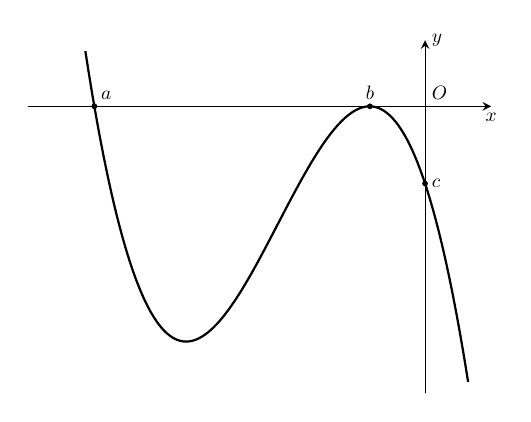
\begin{tikzpicture}[scale=0.7, line join=round, line cap=round, >=stealth]
			\tikzset{every node/.style={scale=.7}}
			\def\xmin{-7}\def\xmax{1}\def\ymin{-5}\def\ymax{1}
			\draw[->] (\xmin-0.2,0)--(\xmax+0.2,0) node[below]{$x$};
			\draw[->] (0,\ymin-0.2)--(0,\ymax+0.2) node[right]{$y$};
			\draw (0,0) node[above right]{$O$};
			\draw (-6,0) node[above right]{$a$} ;\fill (-6,0)circle(1.5pt);
			\draw (-1,0) node[above]{$b$} ;\fill (-1,0)circle(1.5pt);
			\draw (0,-1.4) node[right]{$c$} ;\fill (0,-1.4)circle(1.5pt);
			\clip (\xmin,\ymin) rectangle (\xmax,\ymax);
			\draw[thick,smooth,samples=200,domain=\xmin:\xmax] plot(\x,{0-0.23116184334292986*(\x)^(3.0)-1.8517227910274014*(\x)^(2.0)-3.0221002734458264*(\x)-1.4015393257613549});
	\end{tikzpicture}}
	\loigiai{
		Xét hàm số $u(x)=f(x f(x))-c \Rightarrow g(x)=|u(x)|$, ta đếm số lần đổi dấu của $u(x)$ và $u^{\prime}(x)$.\\
		Ta có $f(x)=k \cdot(x-a)(x-b)^2,$ $\left(\mathop {\lim \limits{n \to +\infty}}\limits_{x\to+\infty}  f(x)=-\infty \Rightarrow k<0\right)$ và có hai điểm cực trị $x=m ;$ $x=b$.\\
		Đường thẳng $y=c$ cắt đồ thị $f(x)$ tại ba điểm phân biệt có hoành độ $\alpha ;$ $\beta ;$ $0$ nên 
		\allowdisplaybreaks
		\begin{eqnarray*}
			&&f(x)-c=k \cdot x(x-\alpha)(x-\beta)\\& \Rightarrow& u(x)=k \cdot x f(x)(x f(x)-\alpha)(x f(x)-\beta).
		\end{eqnarray*}
		Ta có $x f(x)$ đổi dấu khi qua các điểm $x=0 ;$ $ x=a$ và mỗi phương trình $x f(x)=\alpha \Leftrightarrow f(x)=\dfrac{\alpha}{x}$\break $ x f(x)=\beta \Leftrightarrow f(x)=\dfrac{\beta}{x}$ đều có hai nghiệm phân biệt.
		\begin{center}
			\begin{tikzpicture}[scale=0.7, line join=round, line cap=round, >=stealth]
				\tikzset{every node/.style={scale=.7}}
				\def\xmin{-8}\def\xmax{6}\def\ymin{-7}\def\ymax{4}
				\draw[->] (\xmin-0.2,0)--(\xmax+0.2,0) node[below]{$x$};
				\draw[->] (0,\ymin-0.2)--(0,\ymax+0.2) node[right]{$y$};
				\draw (0,0) node[above right]{$O$};
				\draw (-6,0) node[above right]{$a$} ;\fill (-6,0)circle(1.5pt);
				\draw (-1,0) node[above]{$b$} ;\fill (-1,0)circle(1.5pt);
				\draw (0,-1.4) node[above right]{$c$} ;\fill (0,-1.4)circle(1.5pt);
				\clip (\xmin,\ymin) rectangle (\xmax,\ymax);
				\draw[thick,smooth,samples=200,domain=\xmin:\xmax] plot(\x,{0-0.23116184334292986*(\x)^(3.0)-1.8517227910274014*(\x)^(2.0)-3.0221002734458264*(\x)-1.4015393257613549});
				%Vẽ hyperbol
				\draw[line width=1,blue,thick,smooth,samples=200,
				domain=\xmin:-.1] plot(\x,{-5.73/(\x)});
				\draw[line width=1,blue,thick,smooth,samples=200,
				domain=.1:\xmax] plot(\x,{-5.73/(\x)});
				\draw [line width=1,red](\xmin,-1.4)--(\xmax,-1.4);
				\draw (-5.73,-1.4) node[below left]{$\alpha$} ;\fill (-5.73,-1.4)circle(1.5pt);
				\draw (-2.28,-1.4) node[below right]{$\beta$} ;\fill (-2.28,-1.4)circle(1.5pt);
				\draw [dashed](-4.36,0)--(-4.36,-4.27);\fill (-4.36,-4.27)circle(1.5pt);
				\draw (-4.36,0) node[above]{$m$} ;\fill (-4.36,0)circle(1.5pt);
				\draw (-1.75,3.5) node[left]{$y=\dfrac{k}{x},\,(k>0)$};
			\end{tikzpicture}
		\end{center}
		Nên $u(x)$ có $2+2+2=6$ lần đổi dấu.\\
		Xét $u^{\prime}(x)=\left(f(x)+x f^{\prime}(x)\right) \cdot f^{\prime}(x f(x))=0 \Leftrightarrow\hoac{&f(x)+x f^{\prime}(x)=0 \\& x f(x)=m \\& x f(x)=b.}$\\
		Mỗi phương trình $x f(x)=m \Leftrightarrow f(x)=\dfrac{m}{x} ;$ $x f(x)=b \Leftrightarrow f(x)=\dfrac{b}{x}$ có hai nghiệm phân biệt.\\ 
		Và \allowdisplaybreaks
		\begin{eqnarray*}
			f(x)+x f^{\prime}(x)&=&k(x-a)(x-b)^2+k x \cdot\left[(x-b)^2+2(x-a)(x-b)\right]\\
			&=&k(x-b)[(x-a)(x-b)+x(3 x-2 a-b)]\\
			&=&k(x-b)\left[4 x^2-(3 a+2 b) x+a b\right]
		\end{eqnarray*} có ba nghiệm phân biệt.\\
		Nên $u^{\prime}(x)$ có $3+2+2=7$ lần đổi dấu, do đó $u(x)$ có $7$ điểm cực trị.\\ Vậy hàm số $g(x)=|u(x)|$ có $6+7=13$ điểm cực trị.\\
		\mathversion{bold}
		\textit{\textbf{Xem lại số điểm cực trị của hàm tuyệt đối $|u(x)|$}!}\mathversion{normal}
	} 
\end{ex}

%%==========Câu 48
\begin{ex}%[Nguyen Huu Chung Kien]%[Tex hóa Đề Vted 2023] %[2D2G5-5] %Câu 48
	Có bao nhiêu số nguyên $a$ sao cho ứng với mỗi $a$ tồn tại số thực $b$ thoả mãn
	$$
	3^b+4 a^2 \cdot 3^{-b}-\left(\dfrac{5}{3}\right)^b=2 \sqrt{3} a ?
	$$
	\choice 
	{$14$}
	{$6$}
	{\True $7$}
	{$11$}
	\loigiai{
		\begin{itemize}
			\item \textbf{Cách 1.} Biến đối giả thiết thành
			\allowdisplaybreaks
			\begin{eqnarray*}
				&&3^b+4 a^2 \cdot 3^{-b}-\left(\dfrac{5}{3}\right)^b=2 \sqrt{3} a \Leftrightarrow 9^b+4 a^2-5^b=2 \sqrt{3} a \cdot 3^b 
				\\
				& \Leftrightarrow&\left(3^b-\sqrt{3} a\right)^2=5^b-a^2 \Leftrightarrow 3^b-\sqrt{3} a= \pm \sqrt{5^b-a^2}= \pm t,\,(t \geq 0) 
				\\
				& \Leftrightarrow&
				\heva{&\sqrt { 3 } a \pm t = 3 ^  b  \\&
					a ^  2  + t ^  2  = 5 ^  b  }
				\Leftrightarrow \heva{&a=\sqrt{5^b} \sin x \\&
					t=\sqrt{5^b} \cos x \\&
					\sqrt{3} \sin x \pm \cos x=\left(\dfrac{3}{\sqrt{5}}\right)^b\\&x \in\left[-\dfrac{\pi}{2} ; \dfrac{\pi}{2}\right]}\\
				& \Rightarrow& a=\left(\sqrt{5}\right)^{\log \frac{3}{\sqrt{5}}(\sqrt{3} \sin x \pm \cos x)} \sin x \Rightarrow a \in\{0, \ldots, 6\} . \end{eqnarray*}
			\item \textbf{Cách 2.} \allowdisplaybreaks
			\begin{eqnarray*}
				&&4 a^2-2 a \cdot 3^{b+\frac{1}{2}}+9^b-5^b=0 \Rightarrow \Delta_a^{\prime}=3\cdot 9^b-4\left(9^b-5^b\right) \geq 0\\
				&\Leftrightarrow& 9^b \leq 4\cdot 5^b \Leftrightarrow\left(\frac{9}{5}\right)^b \leq 4 \\&\Leftrightarrow& b \leq \log _{\frac{9}{5}} 4 \Rightarrow a^2 \leq 5^b \leq 5^{\log _\frac{9}{5}4} \approx 44,52 \Rightarrow a \in\{ \pm 6, \ldots, 0\}.
			\end{eqnarray*}
			Hoặc đánh giá 
			\allowdisplaybreaks
			\begin{eqnarray*}
				&&3^b=\sqrt{3} a \pm \sqrt{5^b-a^2} \leq \sqrt{(3+1)\left(a^2+5^b-a^2\right)}=\sqrt{4\cdot 5^b}
				\\&\Rightarrow& 9^b \leq 4\cdot 5^b \Leftrightarrow\left(\dfrac{9}{5}\right)^b \leq 4 \Leftrightarrow b \leq \log _{\frac{9}{5}} 4 \\&\Rightarrow& a^2 \leq 5^{\log _\frac{9}{5}4} \approx 44,52 \Rightarrow a \in\{ \pm 6, \ldots, 0\} .
			\end{eqnarray*}
			Ta cần thử lại
			\begin{itemize}
				\item Nếu 
				\allowdisplaybreaks
				\begin{eqnarray*}
					a \in\{-6, \ldots,-1\} &\Rightarrow&\left(3^b+\sqrt{3}\right)^2 \leq\left(3^b-\sqrt{3} a\right)^2=5^b-a^2 \leq 5^b-1.\\
					&&		4 a^2-2 a \cdot 3^{b+\frac{1}{2}}+9^b-5^b \geq 9^b-5^b+2.3^{b+\frac{1}{2}}+4 \\&\Rightarrow& 9^b-5^b+2\cdot 3^{b+\frac{1}{2}}+4 \leq 0.
				\end{eqnarray*}
				Điều này vô lí vì với $b<0 \Rightarrow V T>4-5^b>3>0$ và với $b \geq 0 \Rightarrow V T>9^b-5^b \geq 0$
				\item Nếu $a \in\{0, \ldots, 6\}$ thử trực tiếp (SHIFT SOLVE) nhận. 
			\end{itemize}
			\item \textbf{Cách 3.} Để ý phương trình đã cho là phương trình bậc hai đối với ẩn $a$, vậy
			\allowdisplaybreaks
			\begin{eqnarray*} 
				&&3^b+4 a^2 \cdot 3^{-b}-\left(\dfrac{5}{3}\right)^b=2 \sqrt{3} a \Leftrightarrow 4 a^2-2\cdot 3^{b+\frac{1}{2}} a+9^b-5^b=0 \\
				& \Leftrightarrow& a=\dfrac{3^{b+\frac{1}{2}} \pm \sqrt{3^{2 b+1}-4\left(9^b-5^b\right)}}{4} \Rightarrow a \in\{0, \ldots, 6\}.
			\end{eqnarray*}
		\end{itemize}
	} 
\end{ex}



%Thầy Đoàn Minh Tân
%%==========Câu 49
\begin{ex}%[Đoàn Minh Tân]%[Tex hóa Đề Vted 2023]%[2D4G5-2]
	Xét hai số phức $z_1$, $z_2$ thoả mãn $|z_1-2z_2|=3$ và $|3z_1+z_2|=2$. Khi $|z_1-\sqrt{3}iz_2+i|$ đạt giá trị nhỏ nhất thì $|z_1-z_2|$ bằng
	\choice
	{$\dfrac{17\sqrt{2}}{7}$}
	{\True $\dfrac{2\sqrt{43}}{7}$}
	{$\dfrac{2\sqrt{31}}{7}$}
	{$\dfrac{\sqrt{170}}{7}$}
	\loigiai{
		Đặt $a=z_1-2z_2$ và $b=3z_1+2z_2$, suy ra $z_1=\dfrac{a+2b}{7}$, $z_2=\dfrac{b-3a}{7}$ và $|a|=3$, $|b|=2$.\\
		Khi đó \allowdisplaybreaks
		\begin{eqnarray*}
			P&=&|z_1-\sqrt{3}iz_2+i|=\left|\dfrac{a+2b}{7}-\sqrt{3}i\cdot \dfrac{b-3a}{7}+i\right| \\
			&=&\dfrac{1}{7}\left|a\left(1+3\sqrt{3}i\right)+b\left(2-\sqrt{3}i\right)+7i\right|\\
			&\ge& \dfrac{1}{7}\left[\left|a(1+3\sqrt{3}i)+b(2-\sqrt{3})i\right| -|7i|\right]\\
			&\ge& \dfrac{1}{7}\left[\left|a(1+3\sqrt{3}i)\right|-\left|b(2-\sqrt{3}i)\right|-|7i|\right]\\
			&=&\dfrac{1}{7}\left(6\sqrt{7}-2\sqrt{7}-7\right)=\dfrac{4\sqrt{7}-7}{7}.
		\end{eqnarray*}
		Dấu \lq\lq$=$\rq\rq \, xảy ra khi $\heva{& a\left(1+3\sqrt{3}i\right)=-6\sqrt{7}i\\ &b\left(2-\sqrt{3}i\right)=2\sqrt{7}i.}$\\
		Suy ra $|z_1-z_2|=\left|\dfrac{4a+b}{7}\right|=\dfrac{1}{7}\left|4\left(\dfrac{-6\sqrt{7}i}{1+3\sqrt{3}i}\right)+\dfrac{2\sqrt{7}i}{2-\sqrt{3}i}\right|=\dfrac{2\sqrt{43}}{7}$.
		
	}
\end{ex}

%%==========Câu 50
\begin{ex}%[Đoàn Minh Tân]%[Tex hóa Đề Vted 2023]%[2D3G3-1]
	Cho hàm số $f(x)=x^4+ax^3+bx^2+cx+d$ sao cho hàm số $g(x)=\dfrac{f(x)}{x}$ có bốn điểm cực trị là $-3$; $1$; $\dfrac{4-2\sqrt{13}}{3}$ và $\dfrac{4+2\sqrt{13}}{3}$. Gọi $h(x)$ là hàm số bậc ba có đồ thị đi qua bốn điểm cực trị của hàm số $g(x)$. Diện tích hình phẳng giới hạn bởi hai đường $y=g(x)$, $y=h(x)$ và hai đường thẳng $x=1$, $x=2$ bằng
	\choice
	{$\dfrac{419}{12}-30\ln 2$}
	{$\dfrac{421}{12}-36\ln 2$}
	{\True $\dfrac{587}{12}-36\ln2$}
	{$\dfrac{701}{12}-30\ln2$}
	\loigiai{
		Do $g(x)=\dfrac{f(x)}{x}$ có bốn điểm cực trị là $-3$; $1$; $\dfrac{4-2\sqrt{13}}{3}$ và $\dfrac{4+2\sqrt{13}}{3}$ nên  $$g'(x)=\dfrac{xf'(x)-f(x)}{x^2}=\dfrac{x\left(4x^3+3ax^2+2bx+c\right)-\left(x^4+ax^3+bx^2+cx+d\right)}{x^2}=\dfrac{(x+3)(x-1)\left(3x^2-8x-12\right)}{x^2}.$$
		Các điểm cực trị $(x;y)$ của đồ thị $g(x)$ cùng nằm trên đường cong $y=\dfrac{f'(x)}{(x)'}=f'(x)$.\\
		Do $f'(x)$ là hàm số bậc ba nên $h(x)=f'(x)$.\\
		Suy ra $g(x)=h(x)\Leftrightarrow \dfrac{f(x)-xf'(x)}{x}=0$.\\
		Vậy diện tích hình phẳng giới hạn bởi hai đồ thị hàm số $y=g(x)$ và $y=g(x)$ và hai đường thẳng $x=1$, $x=2$ là
		$$S=\displaystyle\int\limits_1^2\left|g(x)-h(x)\right|\mathrm{\,d}x=\displaystyle\int\limits_1^2\left|\dfrac{(x+3)(x-1)(3x^2-8x-12)}{x}\right|\mathrm{\,d}x=\dfrac{587}{12}-36\ln2.$$
	}
\end{ex}



\Closesolutionfile{ans}
\inputansbox{10}{ans/ans-Vted-17-2023}